\documentclass[ignorenonframetext]{beamer}
\usepackage{beamerthemesplit}
\usepackage{amssymb}

%\documentclass[a4paper]{article}
\usepackage{beamerarticle}
\usepackage{verbatim}

\usepackage{../fhnw-beamer}

%\mode<article>{\usepackage{fullpage}}
%\mode<presentation>{\usetheme{Berlin}}

\date{\today}
\author{rolf.schmutz@fhnw.ch}
\institute{FHNW}
\title {Netzwerke und Datenkommunikation\\B-LS-MI 004\\Physical Layer}


\begin{document} % ===============================================================

\section{NDK B-LS-MI 004: L2}



\begin{frame}
\titlepage
\end{frame}

\begin{frame}
\frametitle{Ziele}
\begin{itemize}
	\item{Repr\"asentation des Quellsignals auf elektromagnetischer Ebene}
	\item{Codierung des Quellsignals (Abgek\"urzt)}
	\item{Verfahren zur Leitungscodierung der Daten aus einem Quellenstrom}
	\item{Techniken in Bezug auf Basisband- und Breitband-Kommunikation (Modulation)}
	\item{Fehlererkennung und -Korrektur}
\end{itemize}
\end{frame}





\begin{frame}
\frametitle{Einfachste Bit-Serielle Daten\"ubertragung}
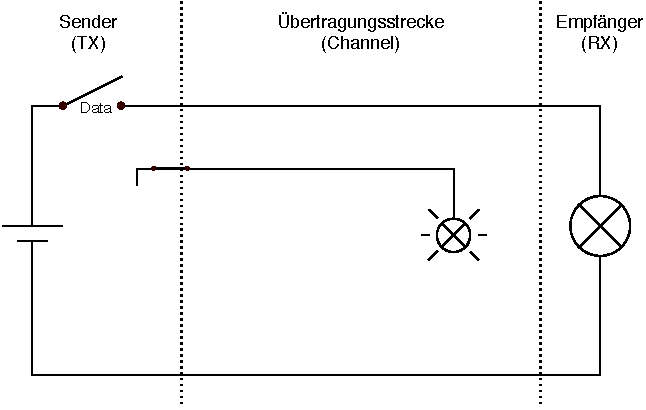
\includegraphics{simplest-serial}

\begin{itemize}
  \item ``Hello World!'' soll \"ubertragen werden
\end{itemize}
\end{frame}
%% Linu/URL/referenz: \myurl{http://www.rfc-editor.org/rfc/pdfrfc/rfc1918.txt.pdf}


\begin{frame}
\frametitle{Probleme}
\begin{itemize}
  \item wie wird ``Hello World!'' als Abfolge von Licht/kein-Licht (0, 1) dargestellt? (Quellcodierung)
  \item wann beginnt die Nachricht, einzelne Buchstaben, einzelne Bits, wann enden sie?
  \item wie k\"onnen einzelne gleiche ``bits'' getrennt werden? z.B. ``o''=01101111
\end{itemize}
\end{frame}


\begin{frame}
\frametitle{Quellencodierung (source-coding) 1/2}
\begin{block}{}
  Das ist die Repr\"asentierung von Informationen in bin\"arer (numerischer) Form, 
  also nicht Programm-Quellcode/sourcecode
\end{block}

\begin{itemize}
  \item es wird eine \"Ubereinkunft/Tabelle ben\"otigt, die die Information in numerischer Form (Bitmuster) festlegt (code-point)
  \item es gibt eine Vielzahl von Codierungen f\"ur verschiedene Datenformate
\end{itemize}
  \begin{block}{}{Die Codierung muss auf beiden Seiten bekannt sein und ist nicht gleich ``Verschl\"usselung''}\end{block}
\end{frame}

\begin{frame}
\frametitle{Quellencodierung (source-coding) 2/2}

F\"ur unsere Zwecke benutzen wir die alterw\"urdige ASCII-Codierungstabelle (ohne Kontrollzeichen):

\begin{center}
\begin{tabular}{l|l}
\begin{minipage}{5cm}
   \begin{tiny}\verbatiminput{asciitable.txt}\end{tiny}
\end{minipage} & z.B. ``H'': 48_{16} = 0100'1000_{2} \\
\end{tabular}
\end{center}

\end{frame}


\begin{frame}
\frametitle{Bit-Synchronisation: Strobe/Clock/Sampling (1/2)}
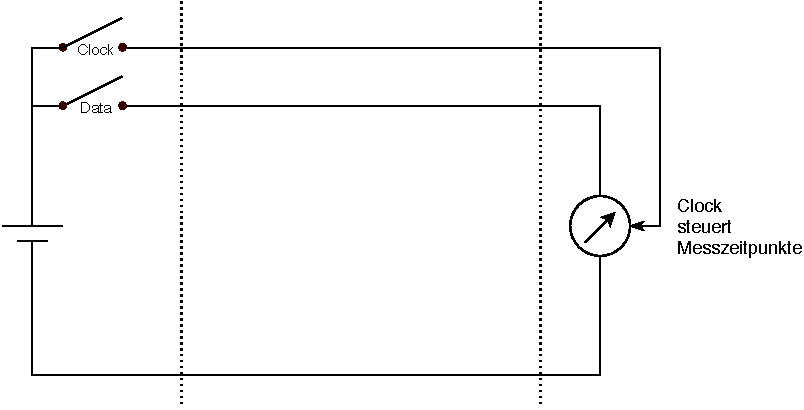
\includegraphics{simplest-serial-clock}
\end{frame}


\begin{frame}
\frametitle{Bit-Synchronisation: Strobe/Clock/Sampling (2/2)}
\begin{itemize}
  \item mit der ``Clock'' Leitung wird dem Empf\"anger der korrekte Messzeitpunkt signalisiert
  \item Folgen von ``gleichen'' Bits (alles 0 oder alles 1) k\"onnen problemlos getrennt werden
\end{itemize}
\begin{block}{Synchrone Bitserielle \"Ubertragung}
Es werden mindestens drei Leitungen ben\"otigt, daf\"ur sind keine weiteren Massnahmen n\"otig.

Synchrone Daten\"ubertragung wird vorallem im Nahbereich (im Computer, Embedded Systems I^{2}C/SPI, HDMI, etc) eingesetzt
\end{block}
\begin{itemize}
  \item es kann auch zwischen ``keine Daten'' (Clock=0) und ``0'' Bits unterschieden werden
\end{itemize}
\end{frame}


\begin{frame}
\frametitle{Asynchrone Serielle \"Ubertragung (1/3)}
Eine weitere M\"oglichkeit eine Synchronisierung\footnote{wenn auch im Titel ``Asynchron''} ist das ``Framing'' der \"Ubertragung

\begin{itemize}
\item eine Startsequenz (Startbit oder Preamble) und eine optionale Endsequenz werden in den Datenstrom eingef\"ugt\footnote{dies sind bereits keine ``Nutzdaten'' mehr sondern Teil des Protokolls}
\item der Empf\"anger hat damit die M\"oglichkeit, sich \emph{f\"ur die Dauer der Nachricht/Zeichens} mit dem Sender zu synchronisieren
\item mit dem Framing kann beim Empf\"anger auch zwischen Daten/keine-Daten unterschieden werden (ausserhalb des Frames werden Daten ignoriert)
\end{itemize}
\begin{block}{Asynchrone Bitserielle \"Ubertragung}
Es werden nur zwei Leitungen/ein Kanal ben\"otigt. Daf\"ur ist die Methode ein wenig aufwendiger zu implementieren.
\end{block}
\end{frame}



\begin{frame}
\frametitle{Asynchrone Serielle \"Ubertragung (2/3)}
Bei einfachen seriellen Schnittstellen (RS232 und \"aquivalent) wird ein Startbit (optional Stopbit) eingef\"ugt:
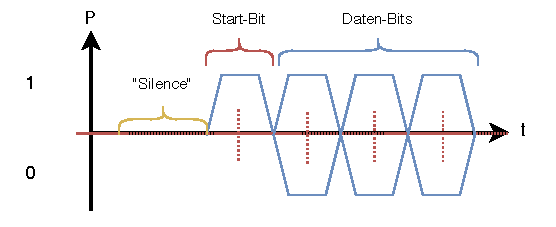
\includegraphics{asynchron-startbit}
\begin{itemize}
\item der Empf\"nger muss ungef\"ahr die Transferrate/Bitzeit schon kennen und kann das Sampling nach dem Startbit einstellen
\item die M\"oglichkeit einer Startsequenz ``10'' vereinfacht dies weiter
\item moderne Implementationen buffern die \"Ubertragung ein paar bits und k\"onnen damit ``autobaud'' -- selbst\"andige Adaption an die Datenrate implementieren
\end{itemize}
\end{frame}


\begin{frame}
\frametitle{Asynchrone Serielle \"Ubertragung (3/3)}
Bei ``Ethernet'' (der Quasi-Standard im Internet/IP-Netzwerken) wird mit einer Pr\"aambel gearbeitet
\begin{itemize}
\item 7 Bytes $AA_{16}$ + 1 Byte $AB_{16}$ {} (d.h. insgesamt 64 Bit)
\item der Empf\"anger hat eine eigene Clock-Source mit der ungef\"ahren Frequenz aber unbekannter Phase. \"Uber eine PLL wird die korrekte Phase ermittelt:
\end{itemize}
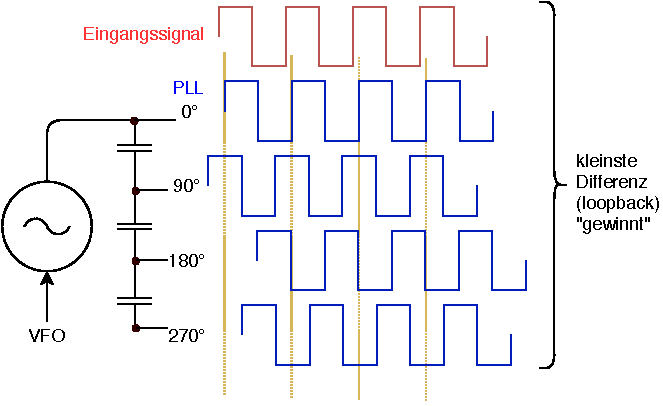
\includegraphics[height=5cm]{asynchron-ethernet}
\end{frame}

\end{document}